\chapter{The Visualization step}
\label{chap:visual}

The goal of the \visual* step is to display the reconstructed 3D particles on a 2D screen, in the most understandable way.
Since no adequate tool was found on the Internet, the Unity renderer (explained in section~\ref{sec:visual:unity}) was initially developed as a versatile, offline tool.
After it was finished, an update to the requirements demanded for a renderer able to display the reconstruction as it was being done: the Open3D renderer (described in section~\ref{sec:visual:o3d}) was then added as an online alternative.

\section{Unity renderer}
\label{sec:visual:unity}

Displayed in figure~\ref{fig:visual:unity}, the Unity renderer is the first visualizer developed in the scope of this thesis.
It is an offline tool, meaning that it is able to show the data after the acquisition is fully processed.
The pipeline produces as output two \texttt{.npz} files, containing the arrays \texttt{positions} and \texttt{validTracers}.
These files can be directly loaded by the Unity scene setup to display their content.

A custom loader was necessary to transform the arrays from the \texttt{NumPy} format into C\# arrays.
Further modules are able to display such arrays in the 3d environment, using simple primitives as backbone.
In particular, the bubbles are represented by spheres in the 3D environment, connected by small rods to display the linked trajectories.

The time evolution of the bubbles is visible with real time: the user is able to ``play'' the scene for inspecting the general behavior.
The user also has control over the time speed, allowing to play back the experiment result in slow-motion, for better observing the fast-moving bubbles.
Alternatively, it is possible for the user to advance or go back by a single frame at a time, allowing to better inspect what happened at the smallest scale of time.

For better understanding the 3D position of the bubbles, the observer is able to move around the simulation.
% The user controls a camera that acts as a 
In particular, the user controls a ``floating camera'' that observes the scene from inside.
It is possible both to rotate the camera around its axes, and to move it.
The movement is possible in the direction where the camera is looking, and in the orthogonal, horizontal direction.
This movement ability allows the user to inspect the reconstruction from whichever angle they prefer.
Figure~\ref{fig:visual:cameradir} displays the way the user can move the visualization camera.

The simulation proposes some more controls to tailor the visualization to the needs of the user.
In particular, it is possible to customize at any time:
\begin{itemize}
	\itemsep 0em
	\item How many frames of trailing trajectory to display: 0, $N$ or all. This allows to concentrate on whatever is required at the moment: a specific time instant, a short-term evolution, or the full history.
	\item The size of the bubbles, that can be reduced up to make them disappear completely. This allows to either focus on the specific time instants where the frames were captured, or on the overall time evolution without focusing on the specific instants.
\end{itemize}

\begin{figure}[H]
	\centerline{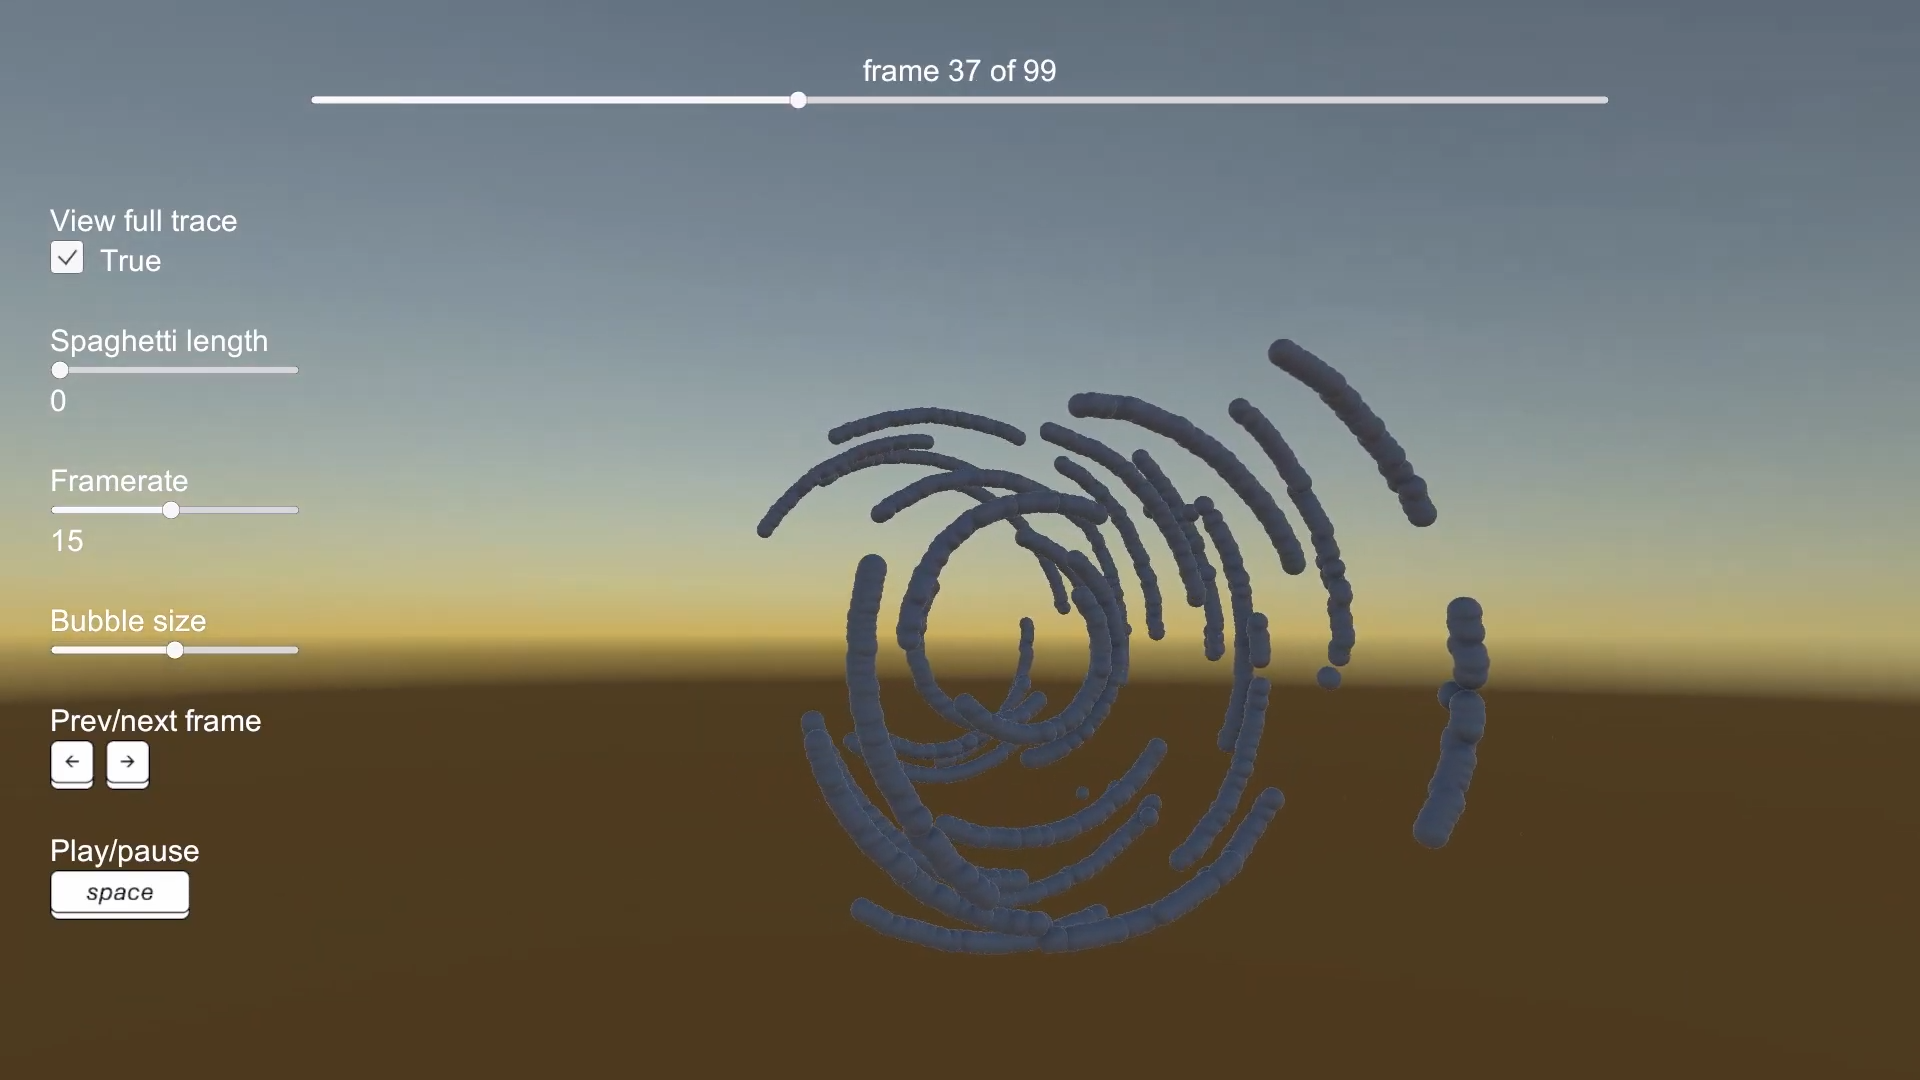
\includegraphics[width=\locateimgsize]{images/visual/unity.png}}
	\caption{\centering An example of bubble visualization using the Unity visualizer. Full video available at~\cite{visual-unity}}
	\label{fig:visual:unity}
\end{figure}

\begin{figure}[H]
	\centering
	\minipage{0.5\textwidth}
	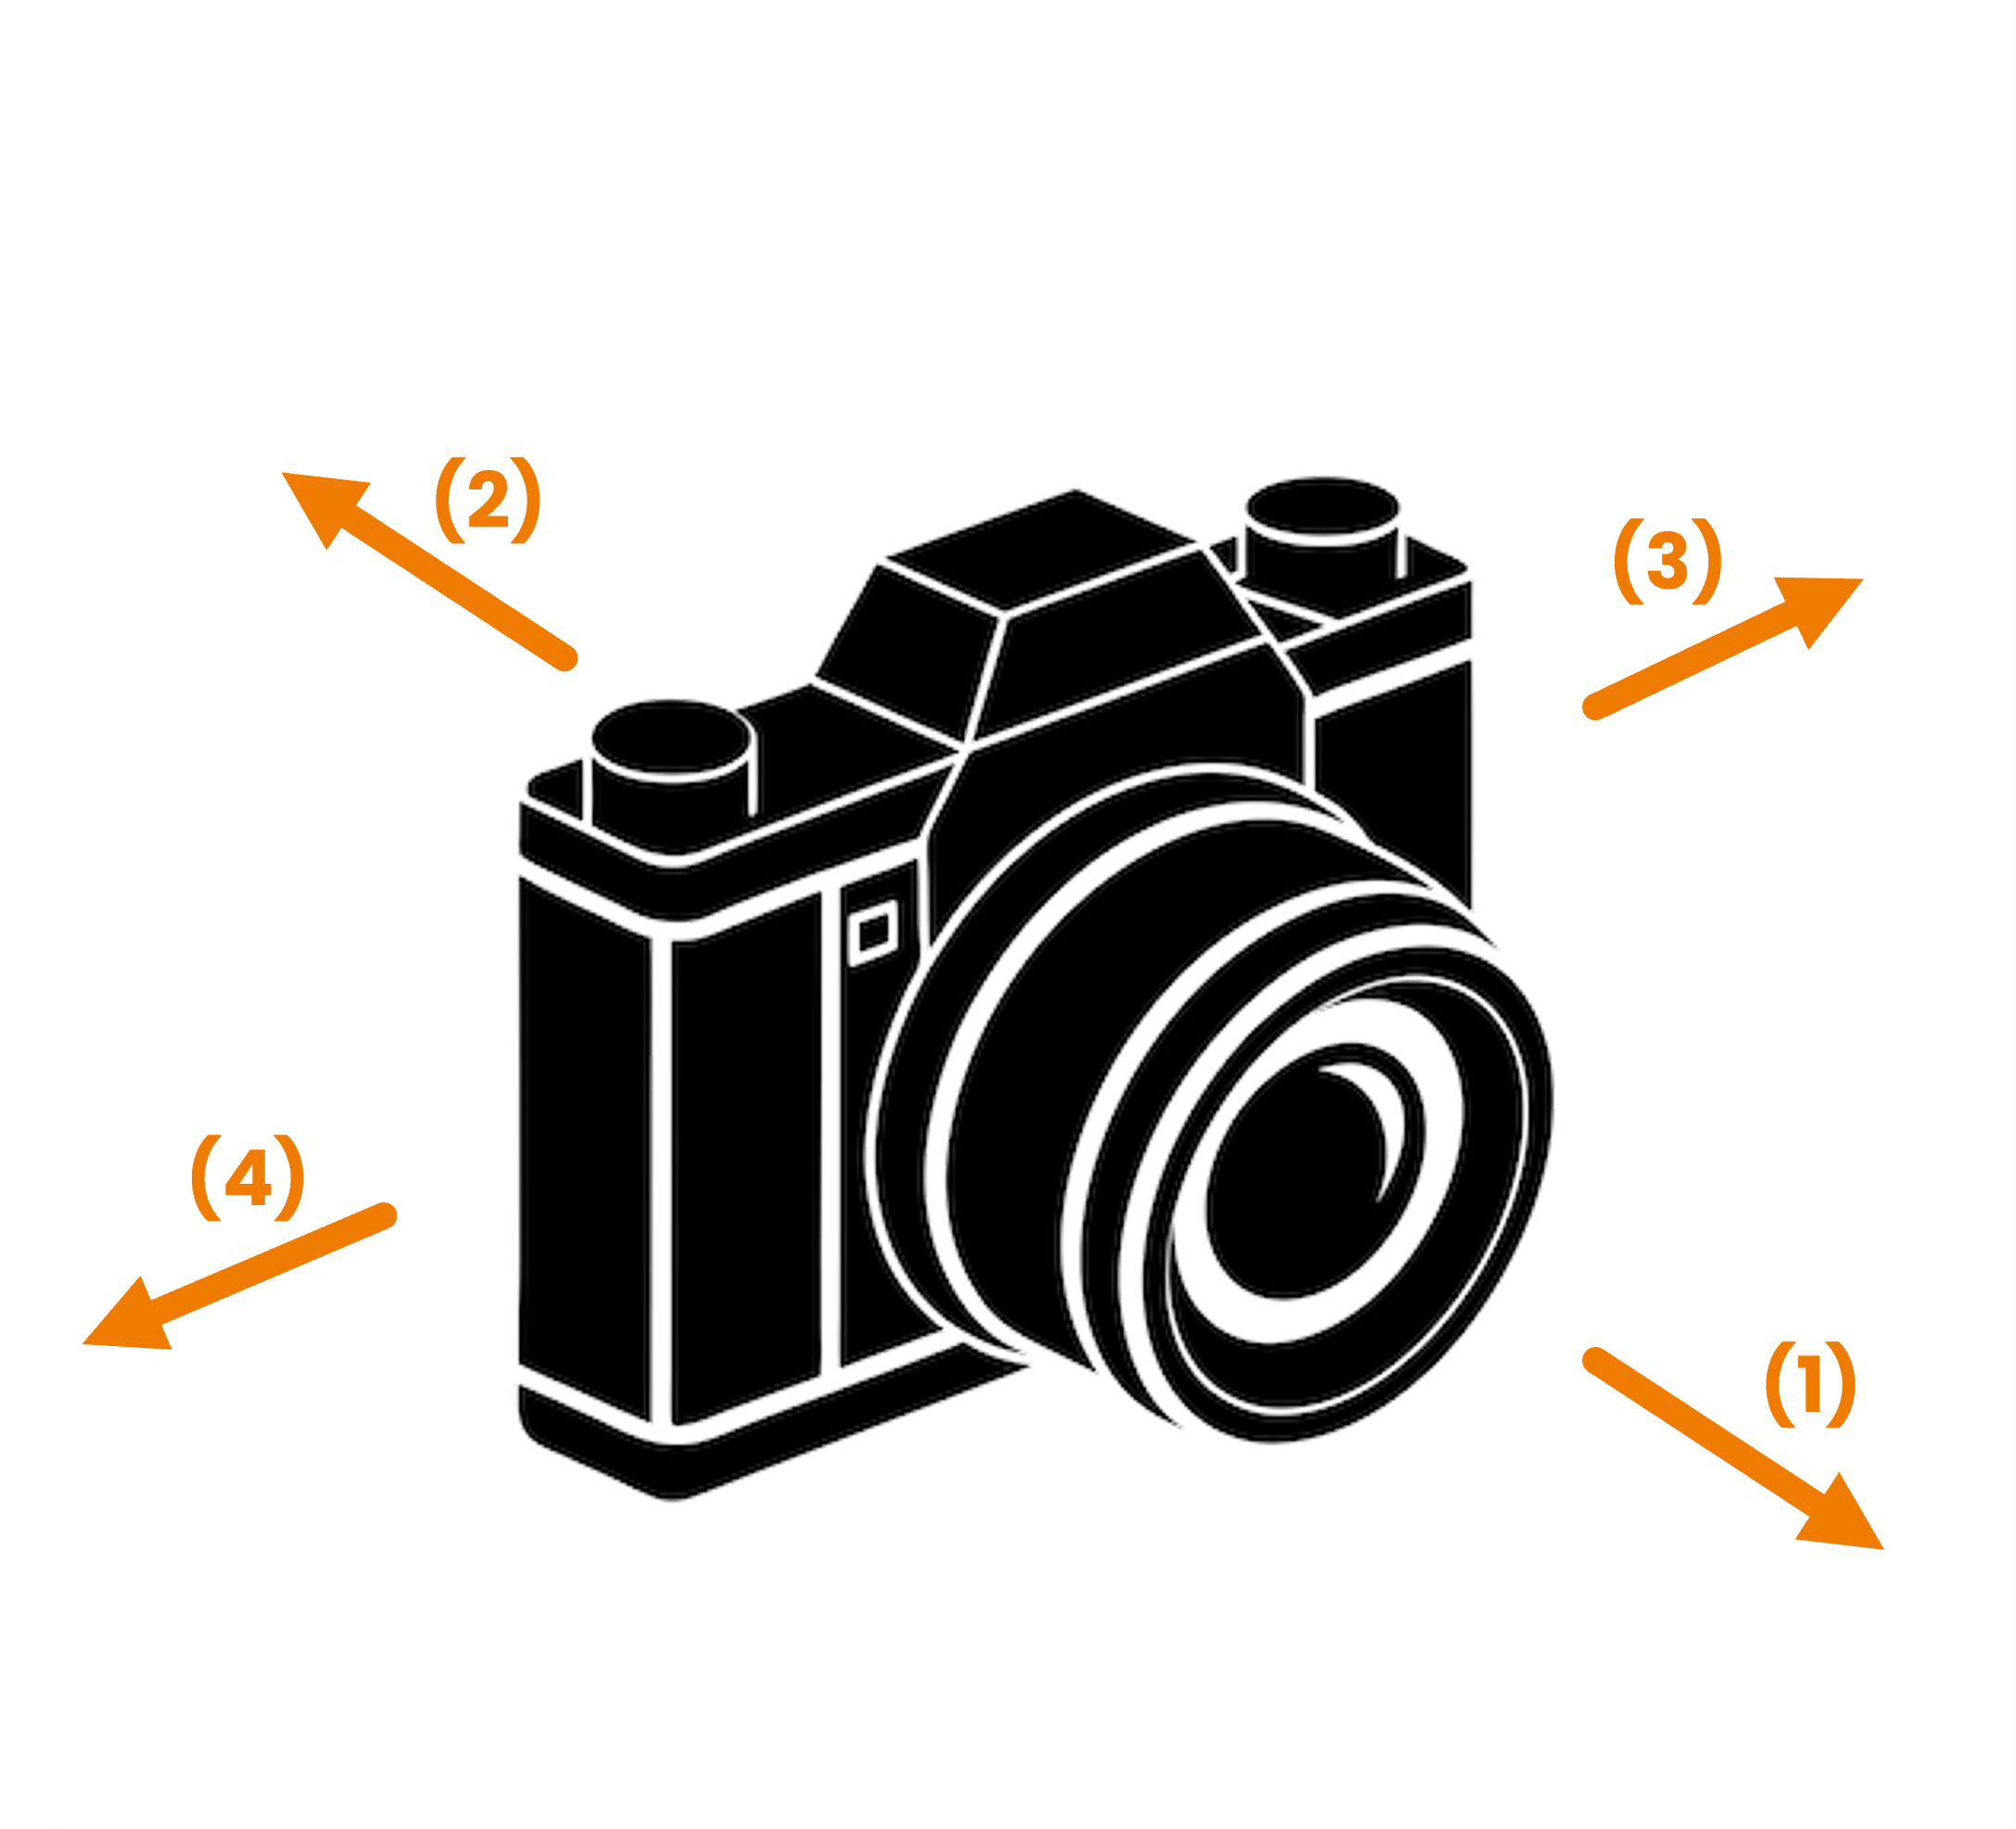
\includegraphics[width=\linewidth]{images/directions-of-moving.png}
	\endminipage\hfill
	\minipage{0.5\textwidth}
	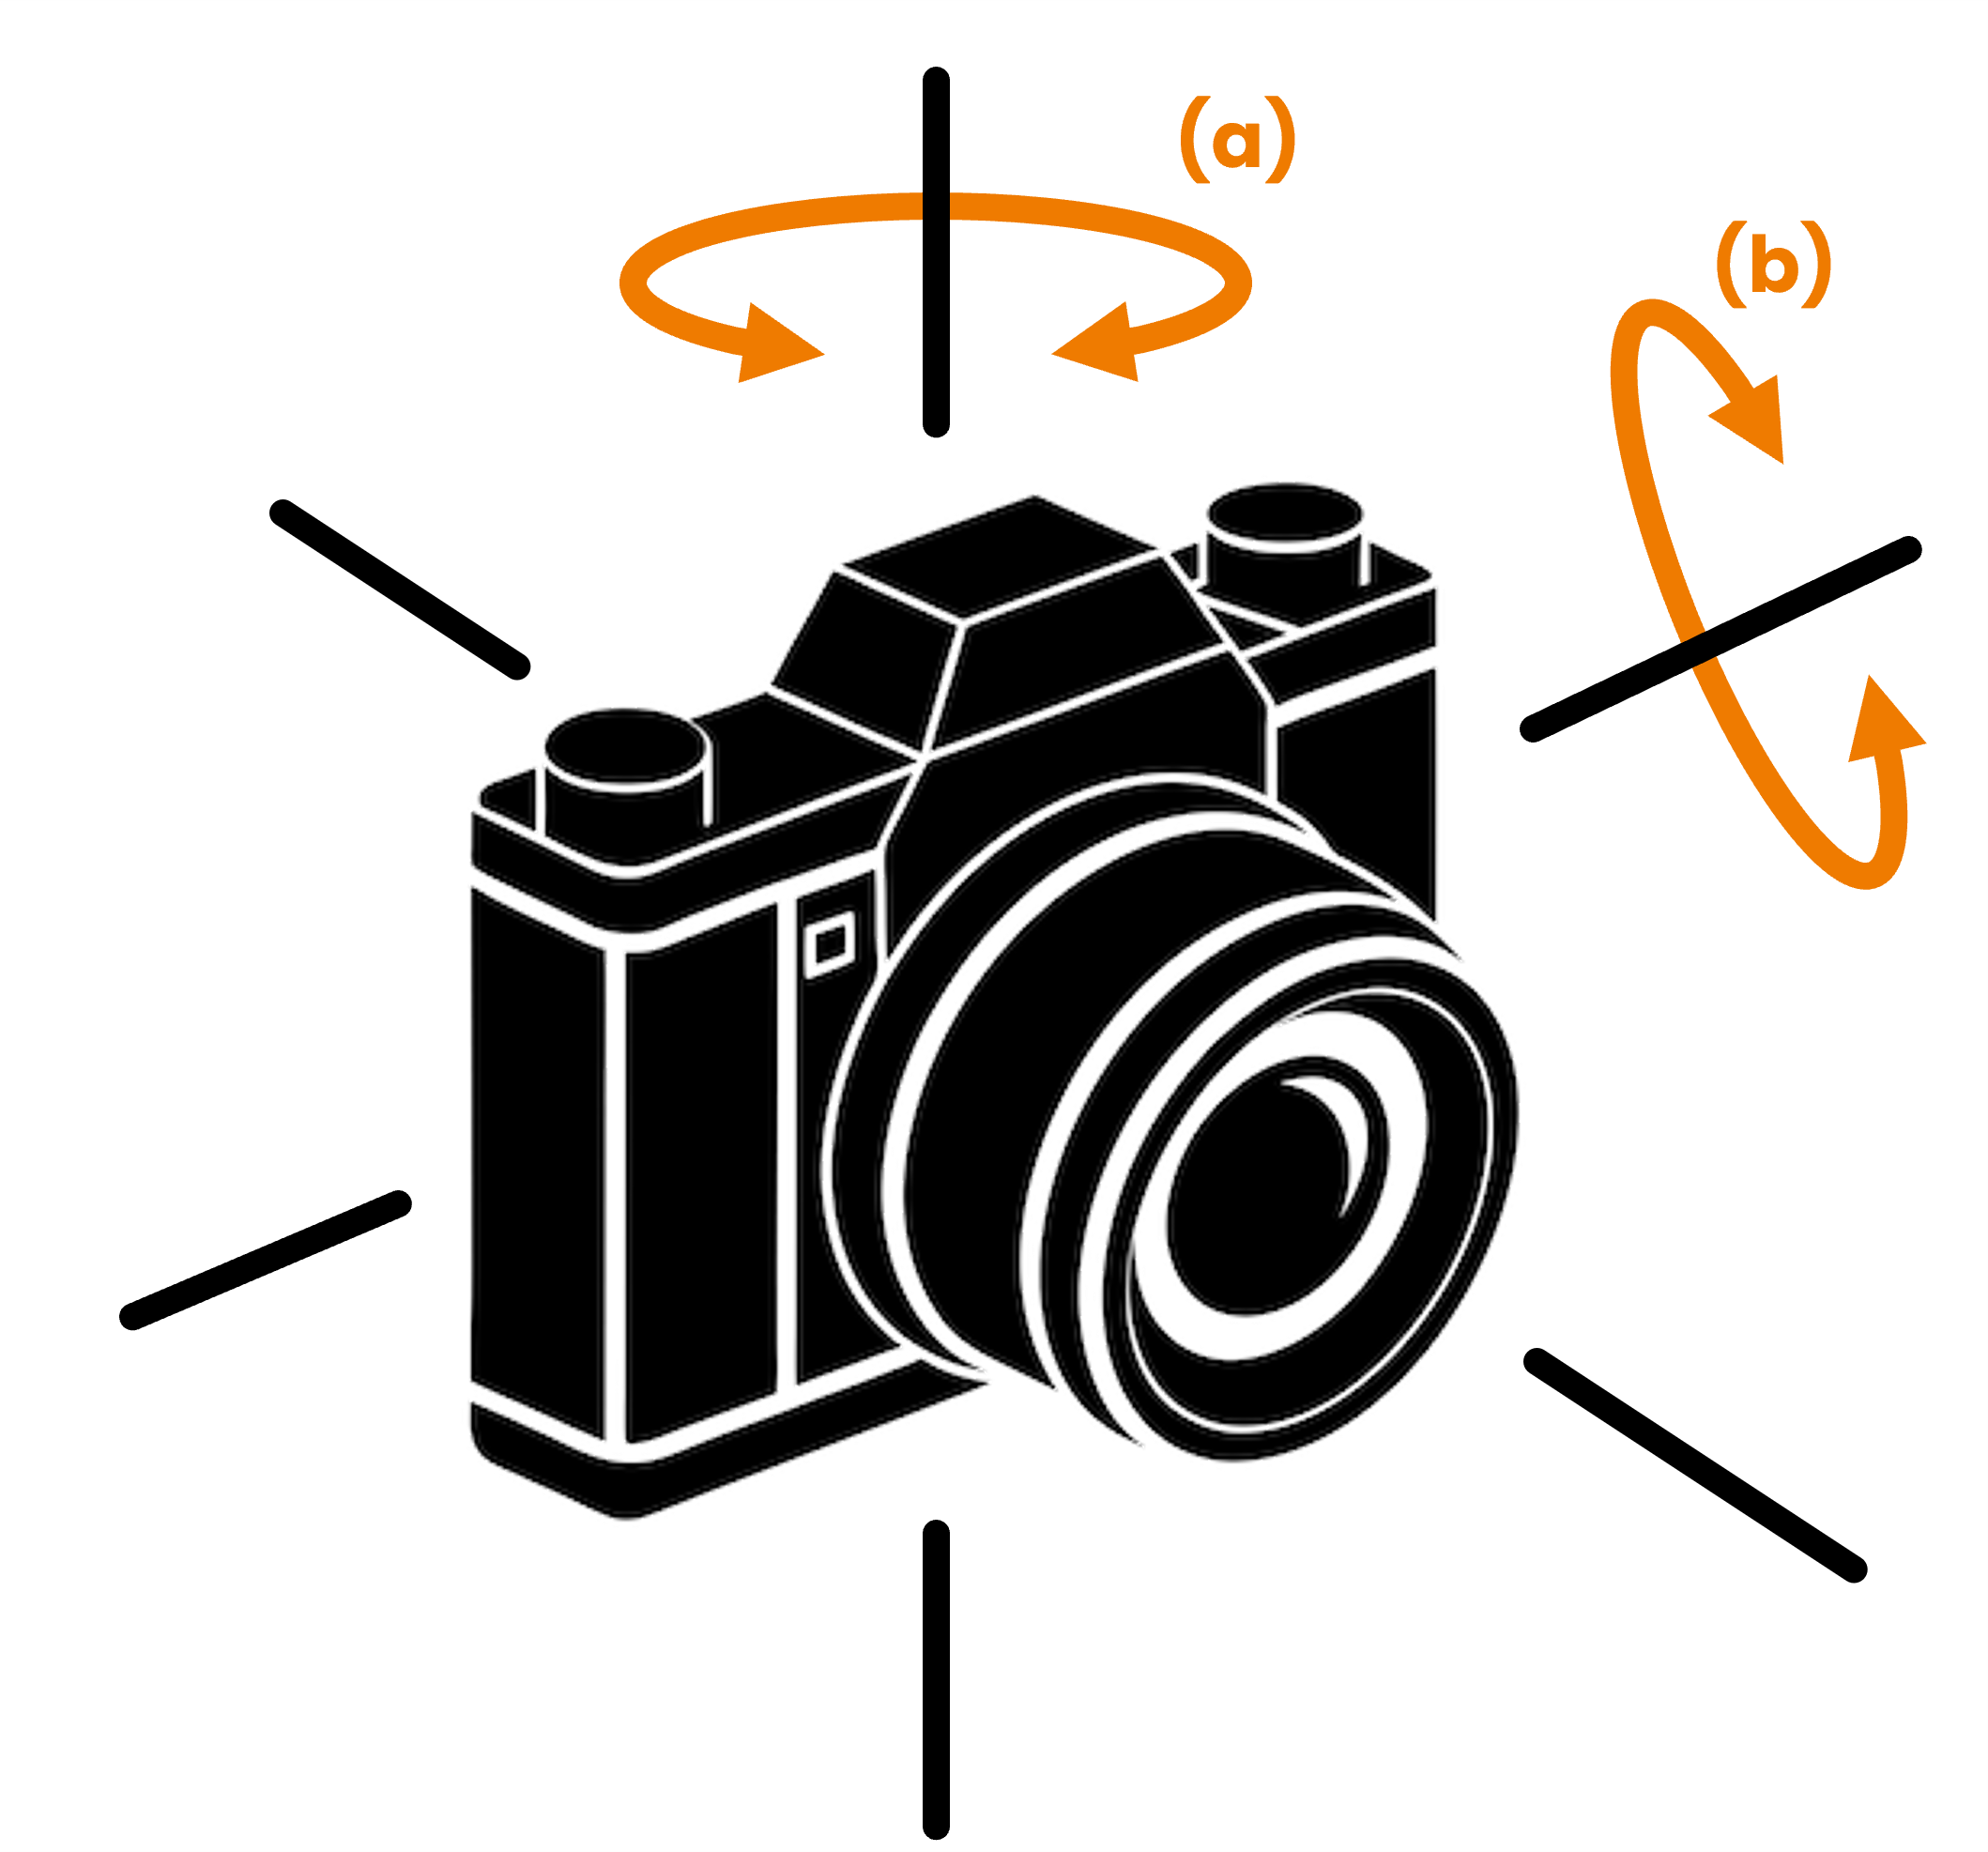
\includegraphics[width=\linewidth]{images/directions-of-rotating.png}
	\endminipage

	\caption{To the left, the four directions in which the user can move the visualization camera: (1) forward, (2) backwards, (3) left and (4) right, with respect of the current ``looking-at'' direction. To the right, the ways it can turn: (a) horizontally or (b) up and down}\label{fig:visual:cameradir}
\end{figure}

\section{Open3D renderer}
\label{sec:visual:o3d}

The Open3D renderer (a screenshot can be seen in figure~\ref{sec:visual:o3d}) was later added, to fulfill the requirements of an online renderer, meaning a renderer that would update in real-time, adding the new bubbles as soon as they are processed.

This was added as a separate step in the pipeline, taking the data directly from the last step.

The user movement is the same as in the Unity renderer (schema available in figure~\ref{fig:visual:cameradir}).
It may however be slightly jumpy, since it's running on an embedded device, which at the same time is executing the rest of the pipeline.

Differently from the Unity renderer, this one cannot use real time as representation of reconstruction time: instead, a color gradient is used, with blue representing the first and red the last time instants.

Another drawback of this visualizer is its volatile nature: displaying the data as soon as it is computed, it is not possible to view back the result once the visualizer is closed.
In such cases, the Unity renderer can be used instead.

\begin{figure}
	\centerline{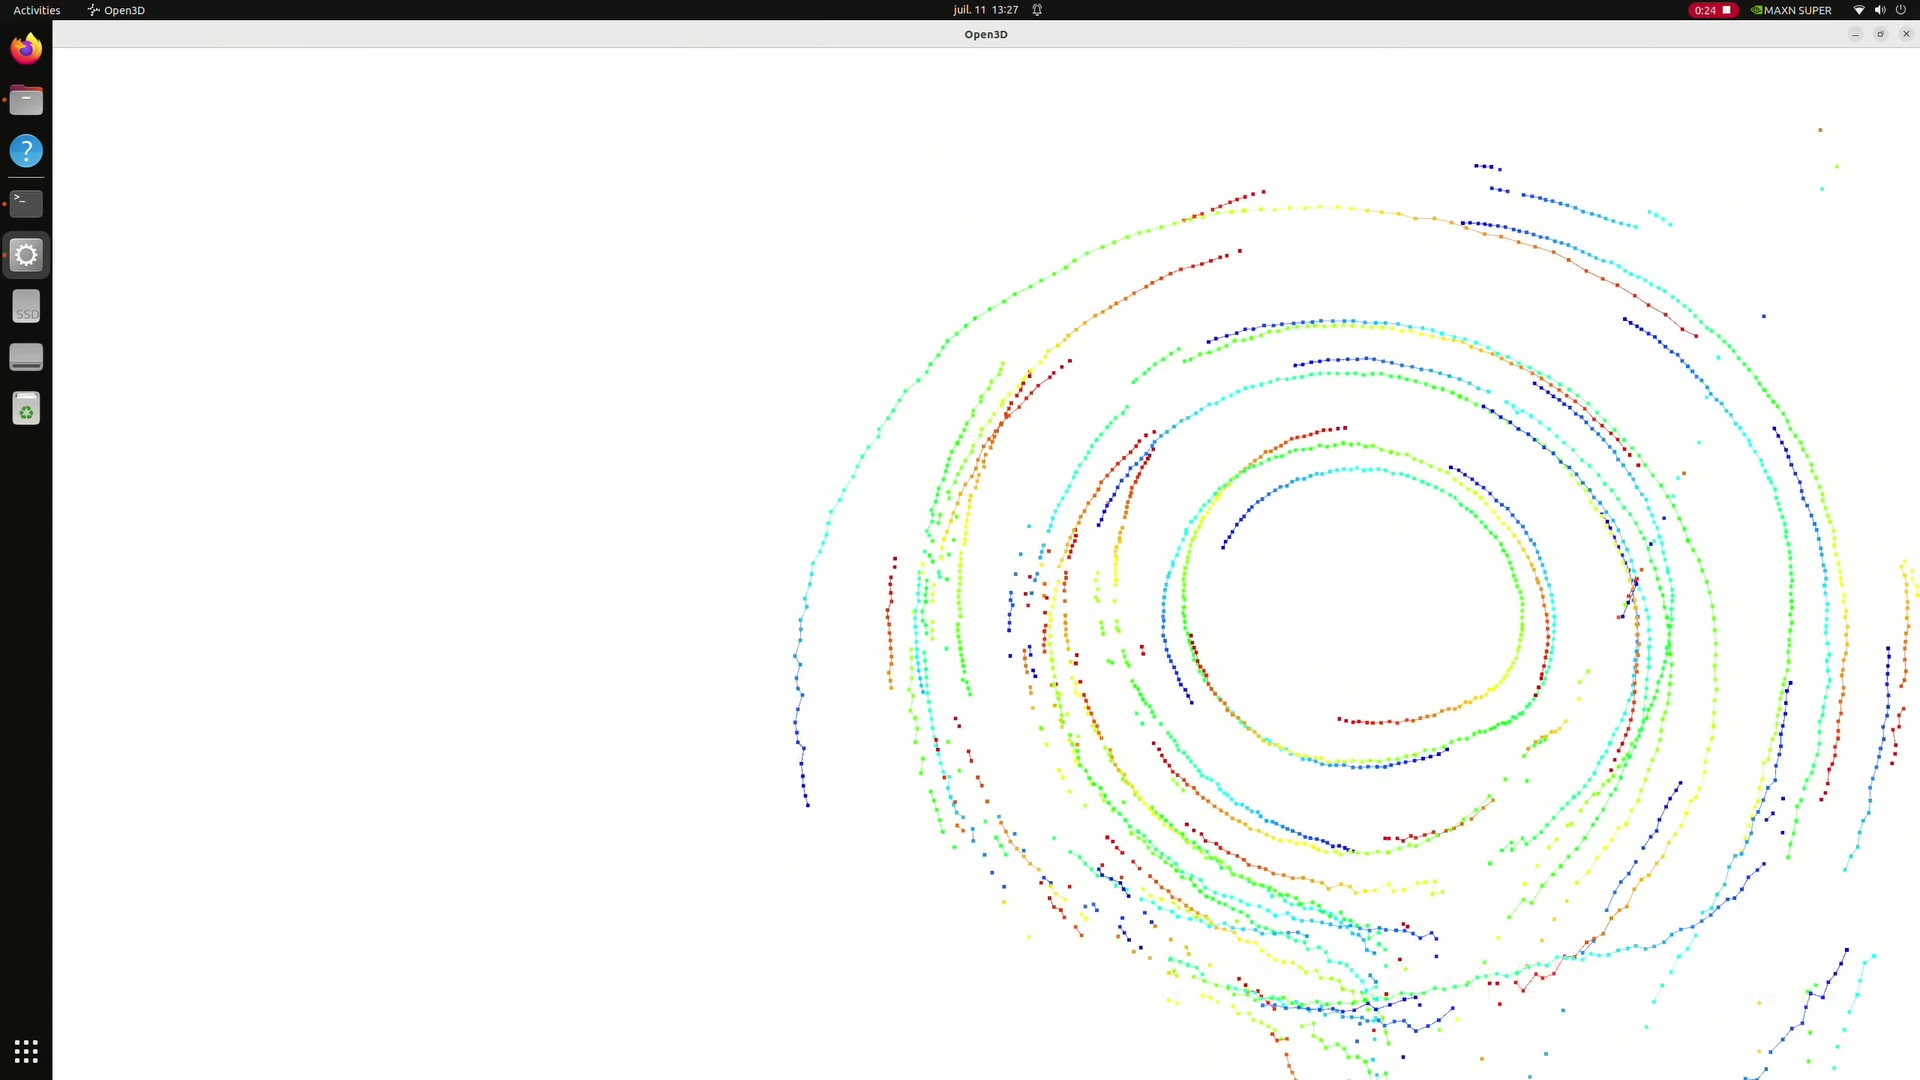
\includegraphics[width=\locateimgsize]{images/visual/o3d.png}}
	\caption{\centering An example of bubble visualization using the Open3D visualizer. Full video available at~\cite{visual-o3d}}
	\label{fig:visual:o3d}
\end{figure}
